\documentclass[11pt]{article}
\usepackage[margin=1in]{geometry}
\usepackage{amsmath,amssymb,amsthm,mathtools}
\usepackage{booktabs,array,microtype,float}
\usepackage{xcolor,hyperref}
\usepackage{tikz}
\usetikzlibrary{arrows.meta,calc}
\usepackage{pgfplots}
\pgfplotsset{compat=1.18}
\definecolor{navy}{HTML}{15324A}
\definecolor{blue}{HTML}{2474A6}
\definecolor{red}{HTML}{B03A2E}
\hypersetup{colorlinks=true,linkcolor=navy,citecolor=navy,urlcolor=blue,pdftitle={A Theoretical Proposal for Amplitude-Phase Composition via a Matrix Method},pdfauthor={German Garcia Andres}}
\newtheorem{definition}{Definition}[section]
\newtheorem{proposition}[definition]{Proposition}
\newtheorem{theorem}[definition]{Theorem}
\newtheorem{corollary}[definition]{Corollary}
\newtheorem{remark}[definition]{Remark}
\renewcommand{\qedsymbol}{}
\newcommand{\Znt}{Z_{\mathrm{nt}}}
\newcommand{\vzero}{\mathbf 0}

\title{\textbf{A Theoretical Proposal for Amplitude--Phase Composition via a Matrix Method}\\[2mm]
\large Multiplicative Amplitude, Additive Phase, and a Prime-Weighted Signal}
\author{German Garcia Andres\\[1mm]\small Independent Researcher}
\date{Final integrated revision, September 8, 2026}

\begin{document}
\maketitle

\begin{abstract}
This note introduces an amplitude--phase state centered on the critical line of the Riemann
zeta function.  For $\rho=\beta+i\gamma$, its normalized amplitude and phase are
$A_\rho(u)=e^{(\beta-1/2)u}$ and $\Phi_\rho(u)=\gamma u+\phi_0$.  The proposed amplitude--phase composition operation
multiplies amplitudes and adds phases:
$(A,\Phi)\star(B,\Psi)=(AB,\Phi+\Psi)$.  Complex multiplication is therefore represented
exactly.  A real $2\times2$ matrix realization converts this composition into ordinary matrix
multiplication, while ordinary complex addition is retained separately for wave superposition and
cancellation.  The quotient of the direct and reflected amplitudes defines the normalized
relative impedance $Z_{\rm RH}=e^{2(\beta-1/2)u}$, with reflection coefficient
$\Gamma_{\rm RH}=(Z_{\rm RH}-1)/(Z_{\rm RH}+1)$.  Unit impedance, zero reflection, and
critical-line fixedness are equivalent for every finite $u>0$.  Log-polar linearization produces the auxiliary Cartesian generator
$(\beta-1/2,\gamma)^T$, whose transverse projection is the signed critical-line defect.
Vanishing of that defect for every nontrivial zero is exactly equivalent to the Riemann
hypothesis.  A second construction expresses each prime power as an amplitude--phase state and
adds its complex carrier to obtain a finite arithmetic vector converging to
$-\zeta'/\zeta$ in $\Re s>1$.  The resulting two-layer compass separates the geometry of zero
localization from the arithmetic prime signal.
\end{abstract}

\begin{center}
\begin{minipage}{0.94\linewidth}
\footnotesize
\textbf{2020 Mathematics Subject Classification.}
Primary 11M26; Secondary 15A24, 30B50.\par
\smallskip
\textbf{Key words and phrases.}
asymptotic wave; amplitude--phase composition; observable structural compression;
matrix formalism; Riemann zeta function; Riemann hypothesis; $\xi$-function;
critical-line symmetry; involution; nodal cancellation; normalized impedance;
commutative composition; prime-weighted angular field.\par
\smallskip
\textbf{Persistent identifiers.}
Primary DOI:
\href{https://doi.org/10.5281/zenodo.22655526}{10.5281/zenodo.22655526};
related Spanish version DOI:
\href{https://doi.org/10.5281/zenodo.22117063}{10.5281/zenodo.22117063}.
\end{minipage}
\end{center}

\section{Purpose and scope}
The word \emph{compass} is used descriptively.  Its primary state has two entries: amplitude
and phase.  These entries do not use the same internal operation.  Amplitude composes by
multiplication and phase composes by addition.  Its log-polar generator is then represented on
two Cartesian axes centered at $\Re s=1/2$.  The construction answers three questions:
\begin{enumerate}
 \item What is the normalized amplitude gain or loss?
 \item What phase is accumulated at ordinate $\gamma$?
 \item How far, and on which side, is the generator from the critical line?
\end{enumerate}
Prime information is then attached through a separate vector obtained from the Euler product.
Keeping these layers distinct is essential: zeros are arguments of an analytic function,
whereas zero vectors and zero matrices are algebraic objects.  The analytic setting follows the
standard theory of the zeta function and its critical strip
\cite{Riemann,Titchmarsh,Bombieri,DLMFzeros}.

The exposition proceeds from coordinates to the amplitude--phase operation and its matrix
realization, then to normalized impedance and the vector criterion.  The prime-weighted layer,
its finite numerical table, and the impedance graph follow afterward; the final sections assemble
the two layers and state the general result.  This order keeps definitions, deductions, and finite
illustrations distinct.

\section{Auxiliary coordinate construction}
Let $q=(q_1,q_2)$ be the tail and $p=(p_1,p_2)$ the head of a directed segment in
$\mathbb R^2$.  Translating the tail to the origin does not change the vector.  Its coordinate
construction is
\begin{equation}\label{eq:displacement}
 \overrightarrow{qp}=p-q
 =\binom{p_1-q_1}{p_2-q_2}
 =(p_1-q_1)\mathbf e_x+(p_2-q_2)\mathbf e_y,
\end{equation}
where
\begin{equation}
 \mathbf e_x=\binom10,\qquad \mathbf e_y=\binom01
\end{equation}
are the standard unit vectors.  For $\mathbf a=(a_1,a_2)^T$,
\begin{equation}\label{eq:norm-direction}
 \|\mathbf a\|=\sqrt{a_1^2+a_2^2},\qquad
 \widehat{\mathbf a}=\frac{\mathbf a}{\|\mathbf a\|}\quad(\mathbf a\ne\vzero_2).
\end{equation}
The zero vector is the unique vector of norm zero in a fixed dimension, and its direction is
undefined.  Vector operations act componentwise:
\begin{equation}
 \mathbf a+\mathbf b=\binom{a_1+b_1}{a_2+b_2},\quad
 \mathbf b-\mathbf a=\binom{b_1-a_1}{b_2-a_2},\quad
 \lambda\mathbf a=\binom{\lambda a_1}{\lambda a_2}.
\end{equation}
These standard facts supply the auxiliary Cartesian representation used below
\cite{HornJohnson,MathInsightVectors}; they do not define the primary amplitude--phase operation.

\section{The RH amplitude--phase vector}
Write $\rho=\beta+i\gamma$, set $x=\beta-1/2$, and let $u>0$ be a finite evolution
parameter.  The associated asymptotic carrier is
\begin{equation}\label{eq:carrier}
 \Psi_\rho(u)=e^{xu}e^{i(\gamma u+\phi_0)}.
\end{equation}

\begin{definition}[RH amplitude--phase vector]\label{def:amplitude-phase}
The primary RH state is the ordered amplitude--phase pair
\begin{equation}\label{eq:amplitude-phase-vector}
 \boxed{
 \mathbf V_\rho(u)
 :=\binom{A_\rho(u)}{\Phi_\rho(u)}
 =\binom{e^{(\beta-\frac12)u}}{\gamma u+\phi_0\pmod{2\pi}}.}
\end{equation}
On $\mathbb R_{>0}\times(\mathbb R/2\pi\mathbb Z)$ define
\begin{equation}\label{eq:star-operation}
 \boxed{(A,\Phi)\star(B,\Psi):=(AB,\Phi+\Psi).}
\end{equation}
Thus the first component multiplies and the second component adds.
\end{definition}

The neutral element and inverse are
\begin{equation}\label{eq:star-neutral-inverse}
 \mathbf 1_\star=(1,0),\qquad
 (A,\Phi)^{\star-1}=(A^{-1},-\Phi).
\end{equation}
The carrier map
\begin{equation}\label{eq:carrier-map}
 \mathcal W(A,\Phi)=Ae^{i\Phi}
\end{equation}
is a group isomorphism onto $\mathbb C^*$:
\begin{equation}\label{eq:carrier-homomorphism}
 \mathcal W\bigl((A,\Phi)\star(B,\Psi)\bigr)
 =\mathcal W(A,\Phi)\mathcal W(B,\Psi).
\end{equation}
This is the usual polar representation of complex multiplication \cite{Ahlfors}.

\subsection{Matrix realization of amplitude and phase}
The matrix method associated with the state $(A,\Phi)$ is the real linear map
\begin{equation}\label{eq:matrix-realization}
 \boxed{
 \mathcal M(A,\Phi)
 :=A\begin{pmatrix}\cos\Phi&-\sin\Phi\\ \sin\Phi&\cos\Phi\end{pmatrix}.}
\end{equation}
It combines a positive dilation of magnitude $A$ with a planar rotation through phase $\Phi$.
Using the angle-addition identities gives
\begin{equation}\label{eq:matrix-composition}
 \mathcal M(A,\Phi)\mathcal M(B,\Psi)
 =AB\begin{pmatrix}
 \cos(\Phi+\Psi)&-\sin(\Phi+\Psi)\\
 \sin(\Phi+\Psi)&\cos(\Phi+\Psi)
 \end{pmatrix}
 =\mathcal M\bigl((A,\Phi)\star(B,\Psi)\bigr).
\end{equation}
Moreover,
\begin{equation}\label{eq:matrix-identity-inverse}
 \mathcal M(1,0)=I_2,\qquad
 \det\mathcal M(A,\Phi)=A^2>0,\qquad
 \mathcal M(A,\Phi)^{-1}=\mathcal M(A^{-1},-\Phi).
\end{equation}
Thus $\mathcal M$ is a faithful real matrix representation of the proposed composition
operation \cite{HornJohnson}; it is the precise sense in which the present construction uses a
matrix method.

Multiplication and wave addition must be distinguished.  The operation $\star$ represents
multiplication of carriers.  Superposition instead uses ordinary complex addition:
\begin{equation}\label{eq:superposition-cancellation}
 \mathcal W(A,\Phi)+\mathcal W(A,\Phi+\pi)=0.
\end{equation}
Hence equal amplitudes and phase opposition produce nodal cancellation, whereas the
proposed amplitude--phase composition operation multiplies amplitudes and adds phases.

Critical reflection $R\rho=1-\overline\rho$ reverses $x$ and preserves $\gamma$, matching the
reflection symmetry of Riemann's completed zeta function \cite{DLMFreflection}.  Therefore
\begin{equation}\label{eq:reflected-state}
 \mathbf V_{R\rho}(u)=\binom{e^{-xu}}{\gamma u+\phi_0},
 \qquad
 \mathbf V_\rho(u)\star\mathbf V_{R\rho}(u)
 =\binom{1}{2(\gamma u+\phi_0)}.
\end{equation}
The product has neutral amplitude for every $x$.  Individual fixedness is stronger:
\begin{equation}\label{eq:state-fixedness}
 \mathbf V_\rho(u)=\mathbf V_{R\rho}(u)
 \iff e^{xu}=e^{-xu}
 \iff x=0
 \iff \beta=\frac12.
\end{equation}

\subsection{Normalized impedance and reflection coefficient}
Within this formalism, \emph{impedance} means the dimensionless relative amplitude of the
direct and reflected branches.  Because both branches have the same phase, the same quantity
is obtained from the quotient of their complex carriers.  The normalized impedance--reflection
transform is used here algebraically in the form introduced for graphical impedance matching
\cite{Smith1939}; no electrical units are assigned to $Z_{\rm RH}$.

\begin{definition}[Normalized RH impedance]\label{def:RH-impedance}
For $u>0$, define
\begin{equation}\label{eq:RH-impedance}
 \boxed{
 Z_{\rm RH}(\rho;u)
 :=\frac{A_\rho(u)}{A_{R\rho}(u)}
 =\frac{\Psi_\rho(u)}{\Psi_{R\rho}(u)}
 =e^{2(\beta-\frac12)u}.}
\end{equation}
The associated normalized reflection coefficient is
\begin{equation}\label{eq:RH-reflection-coefficient}
 \boxed{
 \Gamma_{\rm RH}(\rho;u)
 :=\frac{Z_{\rm RH}(\rho;u)-1}{Z_{\rm RH}(\rho;u)+1}
 =\tanh\!\left[\left(\beta-\frac12\right)u\right].}
\end{equation}
\end{definition}

\begin{theorem}[Unit-impedance criterion]\label{thm:unit-impedance}
For every $\rho=\beta+i\gamma$ and every finite $u>0$, the following statements are
equivalent:
\begin{equation}\label{eq:unit-impedance-equivalence}
 \boxed{
 Z_{\rm RH}(\rho;u)=1
 \iff \Gamma_{\rm RH}(\rho;u)=0
 \iff \mathbf V_\rho(u)=\mathbf V_{R\rho}(u)
 \iff \Re\rho=\frac12.}
\end{equation}
Moreover, the impedance recovers the signed transverse coordinate exactly:
\begin{equation}\label{eq:impedance-inverse}
 \beta-\frac12=\frac{\log Z_{\rm RH}(\rho;u)}{2u}.
\end{equation}
\end{theorem}

\begin{proof}
Since $u>0$ and the real exponential is injective,
\begin{equation}
 Z_{\rm RH}=1
 \iff e^{2(\beta-1/2)u}=1
 \iff \beta-\frac12=0.
\end{equation}
Equation~\eqref{eq:RH-reflection-coefficient} gives
$\Gamma_{\rm RH}=0\iff Z_{\rm RH}=1$, while
\eqref{eq:state-fixedness} gives the state-fixedness equivalence.  Taking the real logarithm
of~\eqref{eq:RH-impedance} yields~\eqref{eq:impedance-inverse}.
\end{proof}

\begin{remark}[Product versus quotient]\label{rem:product-quotient}
The reciprocal product $A_\rho A_{R\rho}=1$ holds for every $\beta$ and therefore does not
detect confinement.  The quotient $A_\rho/A_{R\rho}$ is the discriminating observable: it is
one exactly when the two reciprocal amplitudes are equal.
\end{remark}

\subsection{Log-polar generator and Cartesian projection}
The Cartesian vector is derived from the amplitude--phase state rather than used as its
definition.  Its unwrapped log-polar coordinate is
\begin{equation}\label{eq:log-polar-linearization}
 \mathbf L_\rho(u):=\binom{\log A_\rho(u)}{\Phi_\rho(u)-\phi_0}
 =u\binom{x}{\gamma}.
\end{equation}
Consequently, the rate generator is
\begin{equation}\label{eq:generator}
 \boxed{\mathbf g_{\rm RH}(\rho)
 :=\frac{d}{du}\mathbf L_\rho(u)
 =\binom{\beta-\tfrac12}{\gamma}.}
\end{equation}
This is the auxiliary Cartesian displacement from $c=(1/2,0)$ to
$z_\rho=(\beta,\gamma)$ described in Section~2.

Define the orthogonal projectors
\begin{equation}\label{eq:projectors}
 P_{\parallel}=\begin{pmatrix}0&0\\0&1\end{pmatrix},\qquad
 P_{\perp}=\begin{pmatrix}1&0\\0&0\end{pmatrix}.
\end{equation}
They obey
\begin{equation}
 P_{\parallel}+P_{\perp}=I_2,\quad
 P_{\parallel}P_{\perp}=P_{\perp}P_{\parallel}=O_2,\quad
 P_{\parallel}^2=P_{\parallel},\quad P_{\perp}^2=P_{\perp}.
\end{equation}
Both projectors have rank one.  The critical reflection and the nodal inversion are the
distinct involutions
\begin{equation}\label{eq:critical-nodal-involutions}
 J_c:=P_{\parallel}-P_{\perp}
 =\begin{pmatrix}-1&0\\0&1\end{pmatrix},
 \qquad
 J_n:=-I_2.
\end{equation}
For the centered coordinate vector
$\mathbf a(\rho)=(\beta-\tfrac12,\gamma)^T=\mathbf g_{\rm RH}(\rho)$,
the functional-equation reflection is represented exactly by
\begin{equation}\label{eq:critical-reflection-matrix}
 \mathbf a(R\rho)=J_c\mathbf a(\rho),
 \qquad R\rho=1-\overline\rho.
\end{equation}
Indeed, $R(\beta+i\gamma)=(1-\beta)+i\gamma$, so the transverse coordinate changes
from $\beta-1/2$ to $-(\beta-1/2)$ while the ordinate $\gamma$ is preserved.

\begin{proposition}[Commuting involutions and nodal cancellation]
\label{prop:matrix-commutation}
The matrices $J_c,J_n,P_{\parallel}$ and $P_{\perp}$ commute pairwise.  Moreover,
\begin{align}\label{eq:matrix-commutation}
 J_c^2&=J_n^2=I_2,&
 [J_c,J_n]&=O_2,&
 [P_{\parallel},P_{\perp}]&=O_2,\\
 I_2+J_n&=O_2,&
 \operatorname{rank}(I_2+J_n)&=0.&
\end{align}
Consequently, if two real amplitude vectors are related by phase opposition,
$\mathbf w'=J_n\mathbf w=-\mathbf w$, then
\begin{equation}\label{eq:matrix-nodal-cancellation}
 \mathbf w+\mathbf w'=(I_2+J_n)\mathbf w=O_2\mathbf w=\vzero_2.
\end{equation}
\end{proposition}

\begin{proof}
The matrices in question are diagonal, hence their products are independent of order.
Direct multiplication gives $J_c^2=I_2$, $J_n^2=I_2$ and both commutators equal to
$O_2$.  Since $J_n=-I_2$, one has $I_2+J_n=O_2$, whose image is
$\{\vzero_2\}$ and whose rank is zero.  Multiplication of this identity by $\mathbf w$
gives~\eqref{eq:matrix-nodal-cancellation}.
\end{proof}

The zero matrix and identity matrix therefore have different algebraic roles:
\begin{equation}\label{eq:null-identity-action}
 A+O_2=A,\qquad AO_2=O_2A=O_2,\qquad
 AI_2=I_2A=A
 \quad(A\in M_2(\mathbb R)).
\end{equation}
The projectors are different again: they have rank one and decompose the two-axis state,
whereas $O_2$ has rank zero and $I_2$ has rank two.

\begin{definition}[Longitudinal and defect generators]\label{def:components}
The two projected components are
\begin{align}
 \mathbf v_{\rm RH}(\rho)
  &:=P_{\parallel}\mathbf g_{\rm RH}(\rho)=\binom0\gamma,
  \label{eq:longitudinal}\\
 \mathbf d_{\rm RH}(\rho)
  &:=P_{\perp}\mathbf g_{\rm RH}(\rho)
    =\binom{\beta-\tfrac12}{0}.
  \label{eq:defect}
\end{align}
Thus
\begin{equation}\label{eq:orthogonal-decomposition}
 \mathbf g_{\rm RH}=\mathbf v_{\rm RH}+\mathbf d_{\rm RH},\qquad
 \mathbf v_{\rm RH}^{T}\mathbf d_{\rm RH}=0.
\end{equation}
\end{definition}

\begin{theorem}[Formal two-axis matrix criterion]
\label{thm:formal-matrix-criterion}
For every $\rho=\beta+i\gamma$, the following statements are equivalent:
\begin{equation}\label{eq:formal-matrix-chain}
 \boxed{\begin{aligned}
 J_c\mathbf g_{\rm RH}(\rho)=\mathbf g_{\rm RH}(\rho)
 &\iff P_{\perp}\mathbf g_{\rm RH}(\rho)=\vzero_2\\
 &\iff \|P_{\perp}\mathbf g_{\rm RH}(\rho)\|^2=0\\
 &\iff \beta-\frac12=0
 \iff \Re\rho=\frac12.
 \end{aligned}}
\end{equation}
Equivalently, the fixed sector of $J_c$ is
\begin{equation}\label{eq:fixed-sector}
 \operatorname{Fix}(J_c)=\operatorname{im}P_{\parallel}
 =\left\{\binom0y:y\in\mathbb R\right\}.
\end{equation}
\end{theorem}

\begin{proof}
Writing $x=\beta-1/2$ gives
\begin{equation}
 J_c\binom{x}{\gamma}=\binom{-x}{\gamma},\qquad
 P_{\perp}\binom{x}{\gamma}=\binom{x}{0},\qquad
 \left\|\binom{x}{0}\right\|^2=x^2.
\end{equation}
Thus fixedness under $J_c$, annihilation by $P_{\perp}$, vanishing transverse norm,
and $x=0$ are the same condition.  Substituting $x=\beta-1/2$ gives the remaining
equivalences and~\eqref{eq:fixed-sector}.
\end{proof}

\begin{figure}[H]
\centering
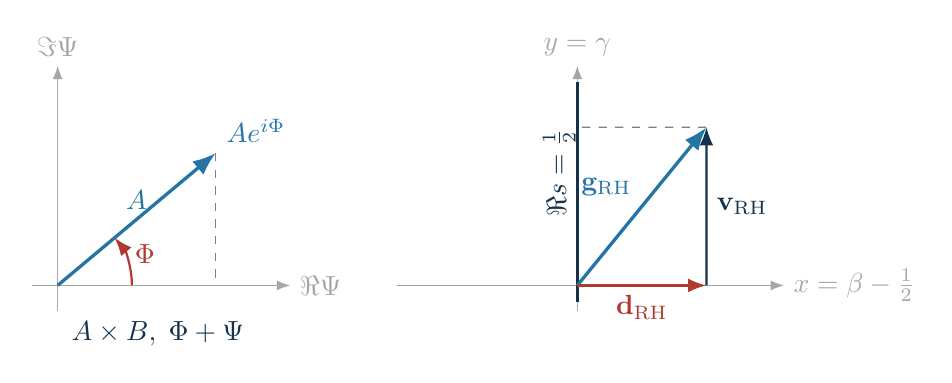
\begin{tikzpicture}[>=Latex]
 \begin{scope}[xshift=-3.5cm,scale=.82]
  \draw[->,gray!70] (-.4,0)--(3.6,0) node[right] {$\Re\Psi$};
  \draw[->,gray!70] (0,-.4)--(0,3.4) node[above] {$\Im\Psi$};
  \draw[->,blue,very thick] (0,0)--(2.45,2.05) node[above right] {$Ae^{i\Phi}$};
  \draw[dashed,gray] (2.45,2.05)--(2.45,0);
  \draw[red,thick,->] (1.15,0) arc[start angle=0,end angle=40,radius=1.15];
  \node[red] at (1.35,.48) {$\Phi$};
  \node[blue] at (1.22,1.32) {$A$};
  \node[navy] at (1.55,-.75) {$A\times B,\;\Phi+\Psi$};
 \end{scope}
 \begin{scope}[xshift=3.1cm,scale=.82]
  \draw[->,gray!70] (-2.8,0)--(3.2,0) node[right] {$x=\beta-\tfrac12$};
  \draw[->,gray!70] (0,-.4)--(0,3.4) node[above] {$y=\gamma$};
  \draw[navy,very thick] (0,-.25)--(0,3.15);
  \coordinate (C) at (0,0); \coordinate (R) at (2.0,2.45);
  \draw[->,blue,very thick] (C)--(R) node[midway,above left] {$\mathbf g_{\rm RH}$};
  \draw[->,red,thick] (C)--(2.0,0) node[midway,below] {$\mathbf d_{\rm RH}$};
  \draw[->,navy,thick] (2.0,0)--(R) node[midway,right] {$\mathbf v_{\rm RH}$};
  \draw[dashed,gray] (R)--(0,2.45);
  \node[navy,rotate=90] at (-.28,1.75) {$\Re s=\tfrac12$};
 \end{scope}
\end{tikzpicture}
\caption{Two representations of the same construction.  Left: the primary state has radial
amplitude $A$ and angular phase $\Phi$; composition multiplies amplitudes and adds phases.
Right: log-polar differentiation produces the auxiliary generator $\mathbf g_{\rm RH}$, whose
horizontal projection is the confinement defect and whose vertical projection is the ordinate.
The direct-to-reflected amplitude ratio is the normalized impedance $Z_{\rm RH}$.}
\label{fig:compass}
\end{figure}

\section{Typed zero objects}
The completed zeta function is
\begin{equation}\label{eq:completed-zeta}
 \xi(s):=\frac12s(s-1)\pi^{-s/2}\Gamma\!\left(\frac{s}{2}\right)\zeta(s),
 \qquad \xi(s)=\xi(1-s).
\end{equation}
Its zeros are precisely the nontrivial zeros of $\zeta$; the reflection identity and complex
conjugation imply invariance under $\rho\mapsto1-\overline\rho$
\cite{Titchmarsh,DLMFreflection,DLMFzeros}.

Four uses of the word \emph{zero} must not be conflated:
\begin{center}
\begin{tabular}{p{0.24\linewidth}p{0.62\linewidth}}
\toprule
Object & Meaning\\
\midrule
$0$ & Scalar additive identity in $\mathbb R$ or $\mathbb C$.\\
$(1,0)$ & Neutral element of the $\star$ amplitude--phase operation; it is not a zero vector.\\
$\vzero_n$ & Unique zero vector in a fixed $n$-dimensional vector space.\\
$O_{m\times n}$ & Zero linear map from $\mathbb C^n$ to $\mathbb C^m$.\\
$\rho$ with $\xi(\rho)=0$ & An argument at which the analytic function $\xi$ vanishes.\\
\bottomrule
\end{tabular}
\end{center}
Their compatible algebra includes
\begin{align}\label{eq:zero-identities}
 \mathbf u+\vzero_n&=\mathbf u,&
 O_{m\times n}\mathbf u&=\vzero_m,\\
 AI_n&=A,& I_mA&=A.
\end{align}
for $\mathbf u\in\mathbb C^n$ and $A\in M_{m\times n}(\mathbb C)$, with the identity sizes
understood.  In particular, $O_2\ne I_2$.  These are standard matrix-space identities
\cite{HornJohnson}.

\section{The exact vector criterion}
Let $\Znt$ denote the multiset of nontrivial zeros of $\zeta$
\cite{Titchmarsh,DLMFzeros}.  By~\eqref{eq:completed-zeta}, this multiset is invariant under
$R\rho=1-\overline\rho$.

\begin{theorem}[RH compass criterion]\label{thm:criterion}
The following statements are equivalent:
\begin{enumerate}
 \item Every $\rho\in\Znt$ satisfies $\Re\rho=1/2$.
 \item $J_c\mathbf g_{\rm RH}(\rho)=\mathbf g_{\rm RH}(\rho)$ for every
 $\rho\in\Znt$.
 \item $\mathbf d_{\rm RH}(\rho)=\vzero_2$ for every $\rho\in\Znt$.
 \item $\mathbf g_{\rm RH}(\rho)=\mathbf v_{\rm RH}(\rho)$ for every
 $\rho\in\Znt$.
 \item $\|\mathbf d_{\rm RH}(\rho)\|^2=0$ for every $\rho\in\Znt$.
 \item $\mathbf V_\rho(u)=\mathbf V_{R\rho}(u)$ for every $\rho\in\Znt$ and one
 (equivalently every) finite $u>0$.
 \item $Z_{\rm RH}(\rho;u)=1$ for every $\rho\in\Znt$ and one
 (equivalently every) finite $u>0$.
 \item $\Gamma_{\rm RH}(\rho;u)=0$ for every $\rho\in\Znt$ and one
 (equivalently every) finite $u>0$.
\end{enumerate}
Equivalently,
\begin{equation}\label{eq:boxed-criterion}
 \boxed{\mathrm{RH}\iff
 \mathbf d_{\rm RH}(\rho)=\vzero_2\quad\text{for all }\rho\in\Znt.}
\end{equation}
\end{theorem}

\begin{proof}
Theorem~\ref{thm:formal-matrix-criterion} and equation~\eqref{eq:defect} give
\begin{equation}
 J_c\mathbf g_{\rm RH}(\rho)=\mathbf g_{\rm RH}(\rho)
 \iff
 \mathbf d_{\rm RH}(\rho)=\vzero_2
 \iff \beta-\frac12=0
 \iff \Re\rho=\frac12.
\end{equation}
Also,
\begin{equation}
 \|\mathbf d_{\rm RH}(\rho)\|^2
 =\left(\beta-\frac12\right)^2,
\end{equation}
which vanishes exactly under the same condition.  Finally,
\eqref{eq:orthogonal-decomposition} gives
$\mathbf g_{\rm RH}=\mathbf v_{\rm RH}$ exactly when
$\mathbf d_{\rm RH}=\vzero_2$.  Applying these pointwise equivalences to all nontrivial
zeros proves the first five equivalences.  The remaining equivalences follow pointwise from
Theorem~\ref{thm:unit-impedance}.
\end{proof}

\subsection{Formal matrix--cell criterion}
The central deductive sequence is
\begin{equation}\label{eq:matrix-cell-sequence}
 \boxed{\begin{gathered}
 \text{coordinates and nodes}
 \longrightarrow \text{Cantor map}
 \longrightarrow \text{matrix symmetries}\\
 \longrightarrow \text{cell invariance}
 \longrightarrow \text{uniqueness}
 \longrightarrow \text{general theorem}
 \longrightarrow \text{corollaries}.
 \end{gathered}}
\end{equation}
For $(i,j)\in\mathbb N_0^2$, the Cantor pairing function
\begin{equation}\label{eq:cantor-cell-map}
 \kappa(i,j)=\frac{(i+j)(i+j+1)}2+j
\end{equation}
is bijective from $\mathbb N_0^2$ to $\mathbb N_0$: for any $k\in\mathbb N_0$, the unique
$w$ satisfying $w(w+1)/2\le k<(w+1)(w+2)/2$ gives
$j=k-w(w+1)/2$ and $i=w-j$.  Thus every two-axis cell label has one and only one scalar
index.

Let $\{B_{ij}\}$ be Jordan cells in the critical strip whose boundaries contain no zero of
$\xi$.  Write
\begin{equation}\label{eq:cell-position-count}
 N(B_{ij})=\#\bigl(\Znt\cap B_{ij}\bigr)
\end{equation}
when zero positions are counted without multiplicity.

\begin{theorem}[General invariant-cell criterion]\label{thm:invariant-cell-general}
Suppose that every occupied cell satisfies
\begin{equation}\label{eq:invariant-unit-cell}
 R(B_{ij})=B_{ij},\qquad N(B_{ij})=1,
\end{equation}
and that the cells cover the nontrivial zero set:
\begin{equation}\label{eq:cell-coverage}
 \Znt\subseteq\bigcup_{i,j}B_{ij}.
\end{equation}
Then
\begin{equation}\label{eq:central-cell-corollary}
 \boxed{
 R(B_{ij})=B_{ij},\quad
 N(B_{ij})=1,\quad
 \Znt\subseteq\bigcup_{i,j}B_{ij}
 \Longrightarrow
 \forall\rho\in\Znt,\quad\Re\rho=\frac12.}
\end{equation}
\end{theorem}

\begin{proof}
Let $\rho\in\Znt$.  Coverage gives a cell $B_{ij}$ containing $\rho$.  Since the zero set is
invariant under $R\rho=1-\overline\rho$ and the cell is also invariant,
$R\rho\in\Znt\cap B_{ij}$.  The equality $N(B_{ij})=1$ leaves only one zero position in
that cell, hence $R\rho=\rho$.  Therefore
\begin{equation}
 1-\overline\rho=\rho
 \iff 1-\Re\rho+i\Im\rho=\Re\rho+i\Im\rho
 \iff \Re\rho=\frac12.
\end{equation}
Equivalently,~\eqref{eq:critical-reflection-matrix} gives
$J_c\mathbf g_{\rm RH}(\rho)=\mathbf g_{\rm RH}(\rho)$, and
Theorem~\ref{thm:formal-matrix-criterion} gives the same conclusion.  Since $\rho$ was
arbitrary, the statement holds for all $\rho\in\Znt$.
\end{proof}

\begin{corollary}[Multiplicity-one cells]\label{cor:simple-zeros}
If the cell count is instead defined by the argument principle,
\begin{equation}\label{eq:cell-multiplicity-count}
 N_{\rm mult}(B_{ij})
 =\frac{1}{2\pi i}\oint_{\partial B_{ij}}\frac{\xi'(s)}{\xi(s)}\,ds,
\end{equation}
and $N_{\rm mult}(B_{ij})=1$ in every occupied cell, then every nontrivial zero is simple.
\end{corollary}

\begin{proof}
The argument principle counts zeros with multiplicity.  A total count equal to one permits
exactly one zero of multiplicity one in each occupied cell.  Coverage applies this conclusion
to every nontrivial zero.
\end{proof}

If, in addition, the occupied cells form a nodal partition in which every zero position is
assigned to exactly one cell, the Cantor index realizes the cell map explicitly:
\begin{equation}\label{eq:explicit-cell-map}
 \mathcal A(\rho)=\kappa(i,j)\quad\text{for }\rho\in B_{ij}.
\end{equation}
Cell invariance gives $\mathcal A(R\rho)=\mathcal A(\rho)$, while unit occupancy gives
injectivity on zero positions.  Hence
\begin{equation}\label{eq:heart-final-chain}
 \boxed{
 \mathcal A(R\rho)=\mathcal A(\rho)
 \ \text{and}\ \mathcal A\ \text{injective}
 \Longrightarrow R\rho=\rho
 \Longrightarrow \Re\rho=\frac12.}
\end{equation}
\section{A finite prime-weighted vector field}
For $s=\sigma+it$ with $\sigma>1$, Euler's product gives the absolutely convergent
identity \cite{Riemann,Titchmarsh,DLMFdefinition}
\begin{equation}\label{eq:log-derivative}
 -\frac{\zeta'(s)}{\zeta(s)}
 =\sum_{p}\sum_{m\ge1}\frac{\log p}{p^{ms}}
 =\sum_p\sum_{m\ge1}\frac{\log p}{p^{m\sigma}}
   e^{-im t\log p}.
\end{equation}
This naturally defines a real planar vector at finite cutoffs.

Each prime power first defines its own amplitude--phase state
\begin{equation}\label{eq:prime-mode-state}
 \mathbf V_{p,m}(\sigma,t)
 :=\binom{(\log p)p^{-m\sigma}}{-mt\log p\pmod{2\pi}},
 \qquad
 \mathcal W(\mathbf V_{p,m})
 =\frac{\log p}{p^{m\sigma}}e^{-imt\log p}.
\end{equation}
Its amplitude is a positive prime weight and its phase is set by the prime frequency
$m\log p$.

\begin{definition}[Prime-weighted arithmetic vector]\label{def:prime-vector}
For $P\ge2$ and $M\ge1$, let
\begin{equation}\label{eq:prime-vector}
 \boxed{
 \mathbf p_{P,M}(\sigma,t)
 :=\sum_{p\le P}\sum_{1\le m\le M}
 \frac{\log p}{p^{m\sigma}}
 \binom{\cos(mt\log p)}{-\sin(mt\log p)}.}
\end{equation}
Its first and second components are respectively the real and imaginary parts of the finite
prime-power sum in~\eqref{eq:log-derivative}.
\end{definition}

The finite truncated vector in~\eqref{eq:prime-vector} is defined for every real $\sigma$;
only the infinite-limit statement requires $\sigma>1$.  For the finite numerical realization
below, set $m=1$, $\sigma=1/2$, and $t=1$.  Then each prime
determines the amplitude and phase
\begin{equation}\label{eq:prime-sample-state}
 a_p=\frac{\log p}{\sqrt p},\qquad
 \phi_p=-\log p\pmod{2\pi}.
\end{equation}
At the same prime-indexed scale $u_p=\log p$, the normalized localization impedance is
\begin{equation}\label{eq:prime-indexed-impedance}
 Z_p(\beta):=Z_{\rm RH}(\beta+it;\log p)=p^{2\beta-1},
 \qquad Z_p\!\left(\frac12\right)=1.
\end{equation}

\begin{table}[H]
\centering
\footnotesize
\caption{Finite prime realization for $m=1$, $\sigma=1/2$, and $t=1$.  The final column
records the common unit-impedance value at $\beta=1/2$.}
\label{tab:prime-amplitude-phase}
\begin{tabular}{rrrrr}
\toprule
$p$ & $u_p=\log p$ & $a_p=(\log p)/\sqrt p$ & $\phi_p$ (rad) & $Z_p(1/2)$\\
\midrule
2  & 0.6931 & 0.4901 & 5.5900 & 1.0000\\
3  & 1.0986 & 0.6343 & 5.1846 & 1.0000\\
5  & 1.6094 & 0.7198 & 4.6737 & 1.0000\\
7  & 1.9459 & 0.7355 & 4.3373 & 1.0000\\
11 & 2.3979 & 0.7230 & 3.8853 & 1.0000\\
13 & 2.5649 & 0.7114 & 3.7182 & 1.0000\\
17 & 2.8332 & 0.6872 & 3.4500 & 1.0000\\
19 & 2.9444 & 0.6755 & 3.3387 & 1.0000\\
23 & 3.1355 & 0.6538 & 3.1477 & 1.0000\\
29 & 3.3673 & 0.6253 & 2.9159 & 1.0000\\
\bottomrule
\end{tabular}
\end{table}

The entries in Table~\ref{tab:prime-amplitude-phase} are direct evaluations of
Equations~\eqref{eq:prime-sample-state}--\eqref{eq:prime-indexed-impedance}, rounded to four
decimal places; they do not use fitted parameters or zero-location data.

\begin{figure}[H]
\centering
\begin{minipage}[t]{0.48\linewidth}
\centering
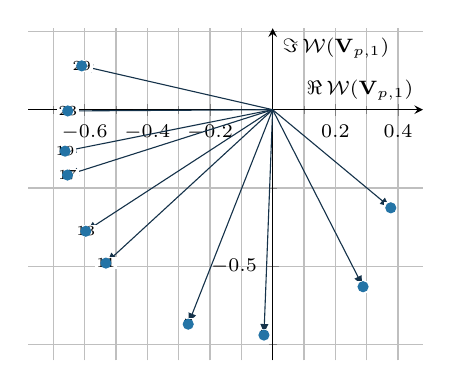
\begin{tikzpicture}
\begin{axis}[
 width=\linewidth,height=5.8cm,
 axis equal image,
 axis lines=middle,
 xmin=-0.78,xmax=0.48,
 ymin=-0.80,ymax=0.26,
 xlabel={$\Re\,\mathcal W(\mathbf V_{p,1})$},
 ylabel={$\Im\,\mathcal W(\mathbf V_{p,1})$},
 tick label style={font=\scriptsize},
 label style={font=\scriptsize},
 grid=both,
 minor tick num=1]
\addplot[blue,only marks,mark=*,mark size=1.8pt] coordinates {
 (0.3770,-0.3132) (0.2885,-0.5649) (-0.0278,-0.7192) (-0.2695,-0.6844)
 (-0.5321,-0.4895) (-0.5964,-0.3879) (-0.6547,-0.2085) (-0.6624,-0.1323)
 (-0.6538,-0.0040) (-0.6094,0.1399)};
\draw[-{Latex[length=1.4mm]},navy,thin] (axis cs:0,0)--(axis cs:0.3770,-0.3132);
\node[font=\tiny,fill=white,inner sep=0.6pt] at (axis cs:0.3770,-0.3132) {2};
\draw[-{Latex[length=1.4mm]},navy,thin] (axis cs:0,0)--(axis cs:0.2885,-0.5649);
\node[font=\tiny,fill=white,inner sep=0.6pt] at (axis cs:0.2885,-0.5649) {3};
\draw[-{Latex[length=1.4mm]},navy,thin] (axis cs:0,0)--(axis cs:-0.0278,-0.7192);
\node[font=\tiny,fill=white,inner sep=0.6pt] at (axis cs:-0.0278,-0.7192) {5};
\draw[-{Latex[length=1.4mm]},navy,thin] (axis cs:0,0)--(axis cs:-0.2695,-0.6844);
\node[font=\tiny,fill=white,inner sep=0.6pt] at (axis cs:-0.2695,-0.6844) {7};
\draw[-{Latex[length=1.4mm]},navy,thin] (axis cs:0,0)--(axis cs:-0.5321,-0.4895);
\node[font=\tiny,fill=white,inner sep=0.6pt] at (axis cs:-0.5321,-0.4895) {11};
\draw[-{Latex[length=1.4mm]},navy,thin] (axis cs:0,0)--(axis cs:-0.5964,-0.3879);
\node[font=\tiny,fill=white,inner sep=0.6pt] at (axis cs:-0.5964,-0.3879) {13};
\draw[-{Latex[length=1.4mm]},navy,thin] (axis cs:0,0)--(axis cs:-0.6547,-0.2085);
\node[font=\tiny,fill=white,inner sep=0.6pt] at (axis cs:-0.6547,-0.2085) {17};
\draw[-{Latex[length=1.4mm]},navy,thin] (axis cs:0,0)--(axis cs:-0.6624,-0.1323);
\node[font=\tiny,fill=white,inner sep=0.6pt] at (axis cs:-0.6624,-0.1323) {19};
\draw[-{Latex[length=1.4mm]},navy,thin] (axis cs:0,0)--(axis cs:-0.6538,-0.0040);
\node[font=\tiny,fill=white,inner sep=0.6pt] at (axis cs:-0.6538,-0.0040) {23};
\draw[-{Latex[length=1.4mm]},navy,thin] (axis cs:0,0)--(axis cs:-0.6094,0.1399);
\node[font=\tiny,fill=white,inner sep=0.6pt] at (axis cs:-0.6094,0.1399) {29};
\end{axis}
\end{tikzpicture}
\par\scriptsize (a) Prime amplitude--phase carriers
\end{minipage}\hfill
\begin{minipage}[t]{0.48\linewidth}
\centering
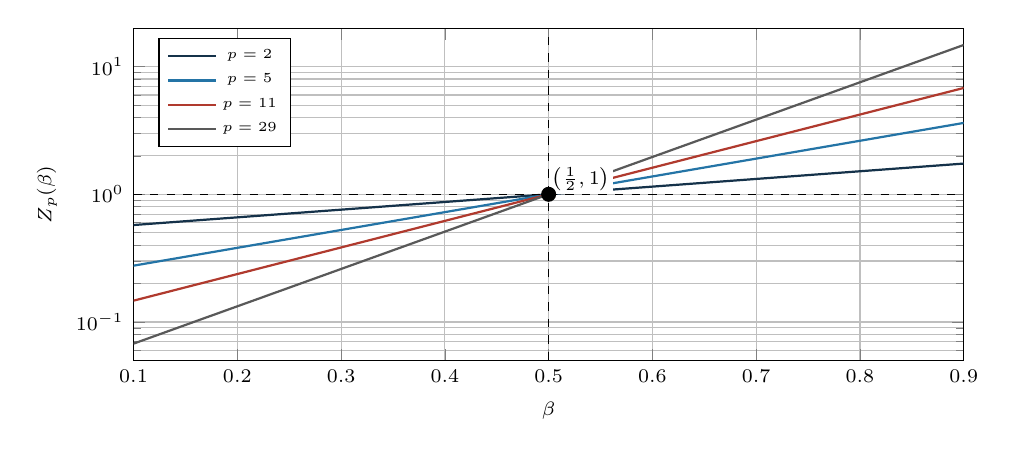
\begin{tikzpicture}
\begin{axis}[
 width=\linewidth,height=5.8cm,
 xmin=0.1,xmax=0.9,
 ymin=0.05,ymax=20,
 ymode=log,
 xlabel={$\beta$},ylabel={$Z_p(\beta)$},
 tick label style={font=\scriptsize},
 label style={font=\scriptsize},
 grid=both,
 legend style={font=\tiny,at={(0.03,0.97)},anchor=north west,fill=white},
 domain=0.1:0.9,samples=80]
\addplot[navy,thick] {exp((2*x-1)*ln(2))};\addlegendentry{$p=2$}
\addplot[blue,thick] {exp((2*x-1)*ln(5))};\addlegendentry{$p=5$}
\addplot[red,thick] {exp((2*x-1)*ln(11))};\addlegendentry{$p=11$}
\addplot[black!65,thick] {exp((2*x-1)*ln(29))};\addlegendentry{$p=29$}
\addplot[black,dashed] coordinates {(0.5,0.05) (0.5,20)};
\addplot[black,dashed] coordinates {(0.1,1) (0.9,1)};
\addplot[black,only marks,mark=*,mark size=2.5pt] coordinates {(0.5,1)};
\node[font=\scriptsize,anchor=south west,fill=white,inner sep=1pt]
 at (axis cs:0.5,1) {$\left(\frac12,1\right)$};
\end{axis}
\end{tikzpicture}
\par\scriptsize (b) Prime-indexed unit-impedance intersection
\end{minipage}
\caption{Prime realization of the amplitude--phase construction.  Left: each labeled prime
defines a carrier with radial amplitude $a_p=(\log p)/\sqrt p$ and angular phase
$\phi_p=-\log p\pmod{2\pi}$.  Right: using $u_p=\log p$, every prime-indexed impedance
$Z_p(\beta)=p^{2\beta-1}$ passes through the common node $(\beta,Z)=(1/2,1)$.  Thus the
direct and reflected normalized amplitudes agree at unit impedance for every displayed prime.}
\label{fig:prime-amplitude-phase-impedance}
\end{figure}

Every summand has amplitude $(\log p)p^{-m\sigma}$ and angular frequency $m\log p$.
Consequently, primes enter as fundamental frequencies and prime powers as their integer
multiples.  Equation~\eqref{eq:prime-vector} is the ordinary vector sum of the real and
imaginary parts of the carriers $\mathcal W(\mathbf V_{p,m})$; it is not the internal
$\star$-product of their amplitude--phase states.  Absolute convergence yields
\begin{equation}\label{eq:prime-vector-limit}
 \lim_{P,M\to\infty}\mathbf p_{P,M}(\sigma,t)
 =\binom{\Re[-\zeta'(s)/\zeta(s)]}{\Im[-\zeta'(s)/\zeta(s)]},
 \qquad \sigma>1,
\end{equation}
where the limit may be taken through any cofinal sequence of cutoffs.

\section{The two-layer compass}
The geometric and arithmetic constructions can be recorded without conflating their domains:
\begin{equation}\label{eq:augmented-compass}
 \mathfrak C_{P,M}(\rho;\sigma,u)
 :=\left(
 \mathbf V_\rho(u),
 Z_{\rm RH}(\rho;u),
 \Gamma_{\rm RH}(\rho;u),
 \mathbf d_{\rm RH}(\rho),
 \mathbf v_{\rm RH}(\rho),
 \mathbf p_{P,M}(\sigma,\gamma)
 \right).
\end{equation}
Here $\rho$ is a zero or zero candidate being geometrically located, while the probe line
$\sigma>1$ is where the prime series converges absolutely.  The common ordinate $t=\gamma$
couples the layers without evaluating the logarithmic derivative at its pole.

The interpretation is exact:
\begin{itemize}
 \item $\mathbf V_\rho$ carries multiplicative amplitude and additive phase;
 \item $Z_{\rm RH}$ and $\Gamma_{\rm RH}$ measure relative mismatch and reflection;
 \item $\mathbf d_{\rm RH}$ gives signed transverse displacement from $\Re s=1/2$;
 \item $\mathbf v_{\rm RH}$ gives longitudinal height;
 \item $\mathbf p_{P,M}$ gives the finite prime-power amplitude and phase at that height.
\end{itemize}
The field can therefore guide a numerical search: scan $t$, compute the finite arithmetic
vector on a safe probe line, and compare its features with independently evaluated values of
$\zeta$.  Such a computation detects numerical patterns; certification of a zero still
requires a rigorous method such as the argument principle.

\section{General amplitude--phase impedance theorem}
\begin{theorem}[General compass closure]\label{thm:general-compass}
Let $S$ be any subset of the critical strip invariant under
$R\rho=1-\overline\rho$, and fix $u>0$.  For each $\rho=\beta+i\gamma\in S$, set
\begin{equation}
 \mathbf V_\rho(u)=\left(e^{(\beta-1/2)u},\gamma u+\phi_0\right),
 \qquad
 (A,\Phi)\star(B,\Psi)=(AB,\Phi+\Psi).
\end{equation}
Then the following statements hold.

\begin{enumerate}
 \item The state space
 $\mathbb R_{>0}\times(\mathbb R/2\pi\mathbb Z)$ is an abelian group under $\star$, and
 $\mathcal W(A,\Phi)=Ae^{i\Phi}$ is an isomorphism from this group to $\mathbb C^*$, while
 $\mathcal M$ in~\eqref{eq:matrix-realization} is a faithful real $2\times2$ representation.

 \item For every $\rho\in S$,
 \begin{equation}\label{eq:general-pointwise-chain}
 \boxed{\begin{gathered}
 \Re\rho=\frac12
 \iff J_c\mathbf g_{\rm RH}(\rho)=\mathbf g_{\rm RH}(\rho)
 \iff \mathbf d_{\rm RH}(\rho)=\vzero_2
 \iff \mathbf V_\rho(u)=\mathbf V_{R\rho}(u),\\
 \mathbf V_\rho(u)=\mathbf V_{R\rho}(u)
 \iff Z_{\rm RH}(\rho;u)=1
 \iff \Gamma_{\rm RH}(\rho;u)=0.
 \end{gathered}}
 \end{equation}

 \item If the equivalent conditions in~\eqref{eq:general-pointwise-chain} hold for every
 $\rho\in S$, then the log-polar generators satisfy
 $\mathbf g_{\rm RH}(S)\subseteq\{0\}\times\mathbb R$.  Thus the coordinate pair reduces
 to $(0,\gamma)$.  The amplitude becomes neutral.  Specifically, $A_\rho(u)=1$, and the
 phase remains $\Phi_\rho(u)=\gamma u+\phi_0$.

 \item For every finite $P,M$ and $\sigma>1$, the prime-power states
 $\mathbf V_{p,m}(\sigma,t)$ realize the arithmetic vector by ordinary carrier
 superposition:
 \begin{equation}\label{eq:general-prime-realization}
  \mathbf p_{P,M}(\sigma,t)
  =\binom{\Re\displaystyle\sum_{p\le P}\sum_{1\le m\le M}
      \mathcal W(\mathbf V_{p,m})}
     {\Im\displaystyle\sum_{p\le P}\sum_{1\le m\le M}
      \mathcal W(\mathbf V_{p,m})}.
 \end{equation}
 As $P,M\to\infty$, this vector converges to the real--imaginary representation of
 $-\zeta'(s)/\zeta(s)$ for $s=\sigma+it$.
\end{enumerate}

In particular, for $S=\Znt$, the universal validity of any condition in
\eqref{eq:general-pointwise-chain} is equivalent to the Riemann hypothesis.
\end{theorem}

\begin{proof}
Associativity, commutativity, the neutral element $(1,0)$, and the inverse
$(A^{-1},-\Phi)$ follow componentwise.  Equations~\eqref{eq:carrier-homomorphism}
and~\eqref{eq:matrix-composition} give the complex and matrix representations.  The
pointwise chain follows from Theorems~\ref{thm:formal-matrix-criterion}
and~\ref{thm:unit-impedance}, together with the definition of $\mathbf d_{\rm RH}$.
Imposing $\beta-1/2=0$ removes the transverse
coordinate and gives the stated amplitude and phase.  Finally,
\eqref{eq:general-prime-realization} is the real--imaginary decomposition of the finite sum
in~\eqref{eq:prime-vector}; its limit is~\eqref{eq:prime-vector-limit}.  Taking
$S=\Znt$ converts $\Re\rho=1/2$ for every $\rho\in S$ into the defining assertion of RH.
\end{proof}

The associated continuous degree-of-freedom count is summarized by
\begin{center}
\begin{tabular}{>{\raggedright\arraybackslash}p{0.39\linewidth}>{\raggedright\arraybackslash}p{0.31\linewidth}c}
\toprule
State & Independent coordinates & DoF\\
\midrule
Amplitude--phase state & $(A,\Phi)$ & $2$\\
Log-polar generator & $(\beta-1/2,\gamma)$ & $2$\\
Unit-impedance fixed sector & $(0,\gamma)$ & $1$\\
Transverse defect after matching & $\mathbf d_{\rm RH}=\vzero_2$ & $0$\\
\bottomrule
\end{tabular}
\end{center}

\section{Conclusion}
The RH compass is fundamentally an amplitude--phase state.  Its proposed composition operation
$(A,\Phi)\star(B,\Psi)=(AB,\Phi+\Psi)$ is realized by ordinary multiplication of the matrices
$\mathcal M(A,\Phi)$ and represents complex multiplication exactly, while
ordinary complex addition represents wave superposition.  Log-polar differentiation then
produces the Cartesian generator $\mathbf g_{\rm RH}$, which decomposes orthogonally into the
height vector $\mathbf v_{\rm RH}$ and the localization-defect vector
$\mathbf d_{\rm RH}$.  Their Pythagorean relation is
\begin{equation}
 \|\mathbf g_{\rm RH}\|^2
 =\|\mathbf v_{\rm RH}\|^2+\|\mathbf d_{\rm RH}\|^2
 =\gamma^2+\left(\beta-\frac12\right)^2.
\end{equation}
The normalized relative impedance and reflection coefficient provide the direct transverse
readout
\begin{equation}
 \boxed{
 Z_{\rm RH}=1
 \iff \Gamma_{\rm RH}=0
 \iff \mathbf V_\rho=\mathbf V_{R\rho}
 \iff \Re\rho=\frac12.}
\end{equation}
Theorem~\ref{thm:general-compass} collects the algebraic, geometric, impedance, degree-of-freedom,
and prime-power layers in one statement, while preserving the distinction between internal
$\star$-composition and ordinary carrier superposition.
The condition $\mathbf d_{\rm RH}=\vzero_2$ for every nontrivial zero is exactly RH.  The
prime-weighted vector is a second object derived from Euler's product; it supplies a rigorous
amplitude--phase signal with frequencies $m\log p$.  The matrix--cell criterion adds the chain
$R(B_{ij})=B_{ij}$, unit positional occupancy, and exhaustive coverage; these hypotheses give
$R\rho=\rho$ for every nontrivial zero, while unit counting by the argument principle also gives
simplicity.  Together, the identities above define the proposed compass as a coherent geometric
and arithmetic formalism.

\microtypesetup{expansion=false}
\begin{thebibliography}{99}
\small
\bibitem{Ahlfors}
L. V. Ahlfors, \emph{Complex Analysis}, 3rd ed., McGraw--Hill, 1979.

\bibitem{Bombieri}
E. Bombieri, ``The Riemann Hypothesis,'' in \emph{The Millennium Prize Problems},
Clay Mathematics Institute and American Mathematical Society, 2006, pp.~107--124.

\bibitem{DLMFdefinition}
NIST Digital Library of Mathematical Functions, \S25.2, ``Definition and Expansions:
Riemann Zeta Function,'' including the Euler product in Eq.~25.2.11,
\url{https://dlmf.nist.gov/25.2}, accessed September 2026.

\bibitem{DLMFreflection}
NIST Digital Library of Mathematical Functions, \S25.4, ``Reflection Formulas:
Riemann Zeta Function,'' \url{https://dlmf.nist.gov/25.4}, accessed September 2026.

\bibitem{DLMFzeros}
NIST Digital Library of Mathematical Functions, \S25.10, ``Zeros: Riemann Zeta Function,''
\url{https://dlmf.nist.gov/25.10}, accessed September 2026.

\bibitem{HornJohnson}
R. A. Horn and C. R. Johnson, \emph{Matrix Analysis}, 2nd ed.,
Cambridge University Press, 2013.

\bibitem{MathInsightVectors}
D. R. Wilkins and contributors, ``Vectors in Cartesian coordinates in two and three
dimensions,'' \emph{Math Insight}, University of Minnesota,
\url{https://mathinsight.org/vectors_cartesian_coordinates_2d_3d}, accessed 2026.

\bibitem{Riemann}
B. Riemann, ``Ueber die Anzahl der Primzahlen unter einer gegebenen Gr\"osse,''
\emph{Monatsberichte der K\"oniglich Preussischen Akademie der Wissenschaften zu Berlin},
1859, pp.~671--680.

\bibitem{Smith1939}
P. H. Smith, ``Transmission Line Calculator,'' \emph{Electronics}, vol.~12, no.~1,
January 1939, pp.~29--31.

\bibitem{Titchmarsh}
E. C. Titchmarsh, revised by D. R. Heath-Brown,
\emph{The Theory of the Riemann Zeta-Function}, 2nd ed., Oxford University Press, 1986.
\end{thebibliography}

\end{document}
